\documentclass[aspectratio=169,11pt]{beamer}

\usetheme{Madrid}
\usecolortheme{seahorse}
\usepackage[utf8]{inputenc}
\usepackage[T1]{fontenc}
\usepackage{graphicx}
\usepackage{booktabs}
\usepackage{amsmath}
\usepackage{xcolor}
\providecommand{\degree}{^{\circ}}

\setbeamertemplate{navigation symbols}{}
\setbeamertemplate{footline}[frame number]

\title{License Plate Deblurring}
\subtitle{A Critical Evaluation of Classical Blind Deconvolution}
\author{Hamza Ziouine \and Leonce Theureau}
\institute{Universit\'e Internationale de Rabat --- Group Opus}
\date{April 2026}

\begin{document}

% ---- 1: Title ----
\begin{frame}
\titlepage
\end{frame}

% ---- 2: Problem & Scope ----
\begin{frame}{Problem \& Scope}
\textbf{Problem.} Surveillance plate images are blurred
(motion, defocus, atmospheric). \\[0.2cm]

\textbf{Degradation model:} \quad $y = k \ast x + n$ \\[0.2cm]

\textbf{Scope of this work.} Classical, learning-free image-fidelity pipeline:

\vspace{0.2cm}
\begin{center}
\small
\fbox{Blurry Image} $\rightarrow$
\fbox{FFT PSF Est.} $\rightarrow$
\fbox{Deconvolution} $\rightarrow$
\fbox{PSNR / SSIM}
\end{center}

\vspace{0.3cm}
\textbf{Out of scope (discussed as future work):} OCR / CER evaluation,
TV quantitative ablation, learned priors.
\end{frame}

% ---- 3: Dataset ----
\begin{frame}{Dataset}
\begin{columns}
\begin{column}{0.55\textwidth}
\textbf{Synthetic paired data} (perfect ground truth):
\begin{itemize}
  \item 1\,001 clean plates $\times$ 3 blur types = \textbf{3\,003 pairs}
  \item Gaussian ($\sigma \in [1,5]$), motion ($5$--$25$\,px), defocus ($r \in [3,10]$\,px)
  \item + additive noise ($\sigma \leq 15$) + JPEG ($q \in [50, 85]$)
  \item Split by source image $\Rightarrow$ no leakage
\end{itemize}
\end{column}
\begin{column}{0.4\textwidth}
\begin{tabular}{lr}
\toprule
Split & Images \\
\midrule
Train & 2\,100 \\
Validation & 450 \\
Test & 453 \\
\midrule
\textbf{Total} & \textbf{3\,003} \\
\bottomrule
\end{tabular}
\end{column}
\end{columns}
\end{frame}

% ---- 4: Blind PSF Estimation ----
\begin{frame}{Blind PSF Estimation via FFT}
\textbf{Assumption:} motion blur. (We revisit this in slide 8.) \\[0.2cm]

\begin{enumerate}\setlength{\itemsep}{2pt}
  \item Magnitude spectrum $|F(u,v)|$ of blurry image (log-scaled, fftshifted)
  \item \textbf{Angle:} 1\textdegree\ radial sweep --- minimum-energy direction = blur angle
  \item \textbf{Length:} null spacing along dark band --- $L \approx N / \Delta$
\end{enumerate}

\vspace{0.2cm}
\begin{figure}
\centering
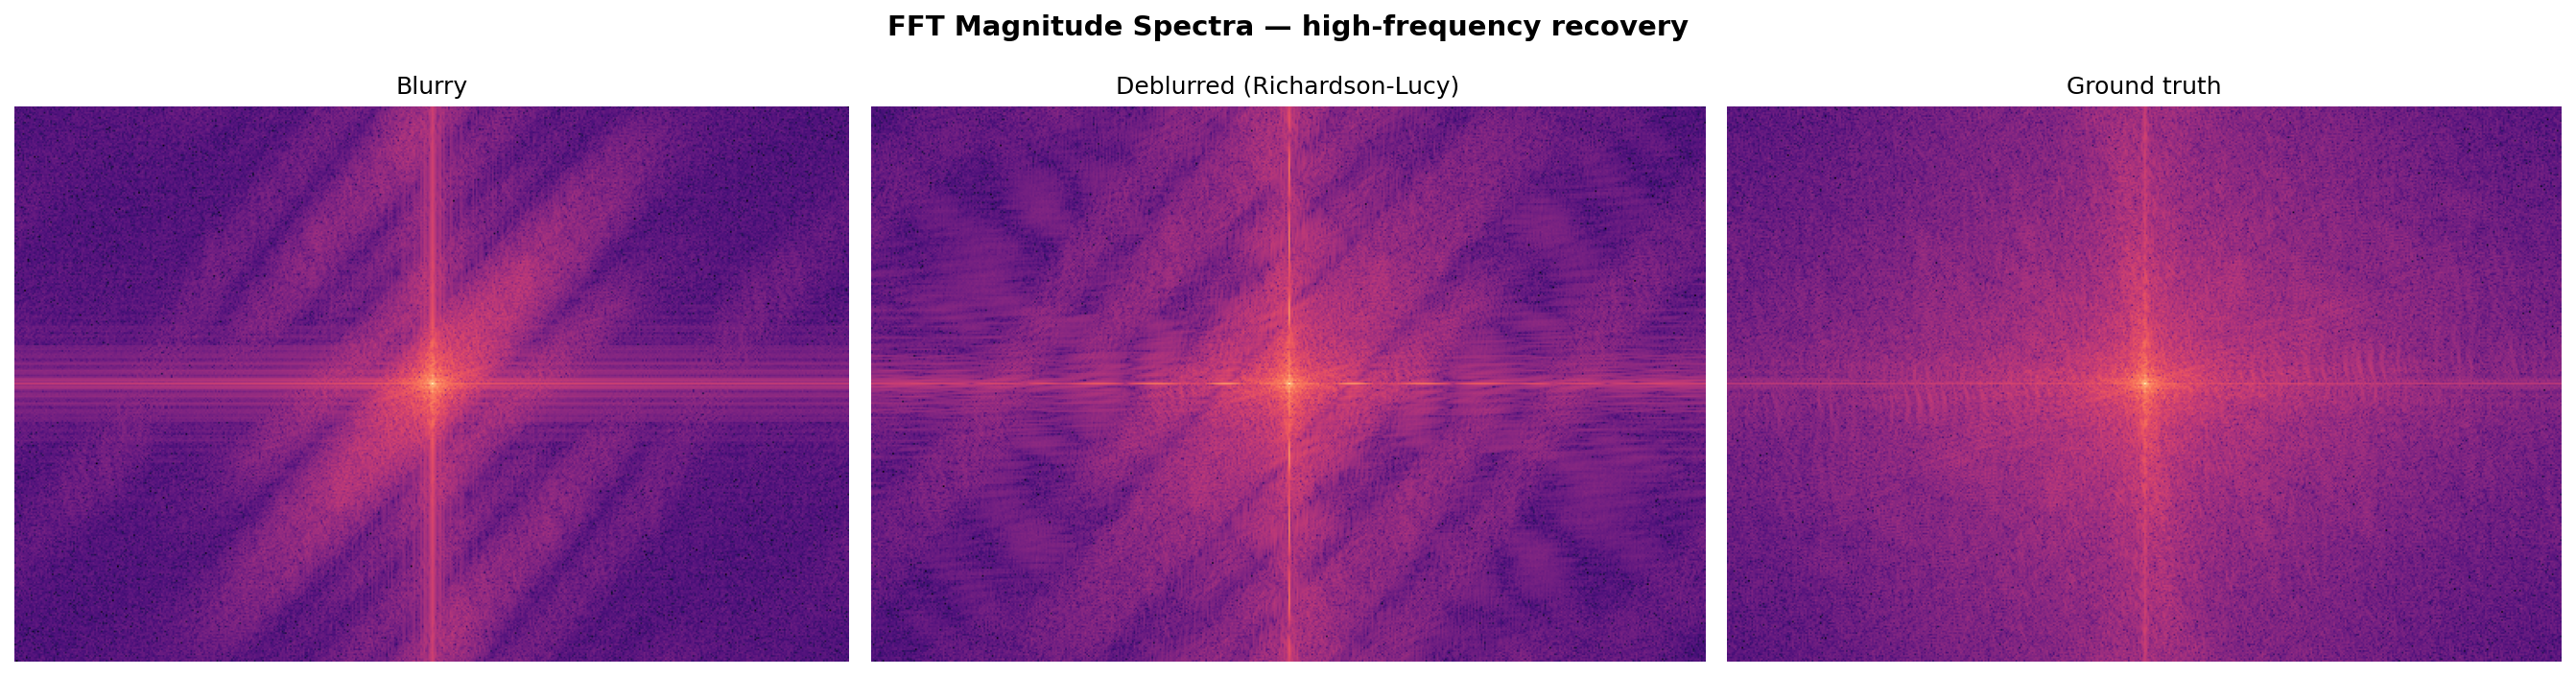
\includegraphics[width=0.65\textwidth,height=0.4\textheight,keepaspectratio]{../outputs/figures/fft_analysis.png}
\caption{\small Blur attenuates high frequencies along the motion direction}
\end{figure}
\end{frame}

% ---- 5: Deconvolution Methods ----
\begin{frame}{Five Deconvolution Methods}
\small
\begin{enumerate}\setlength{\itemsep}{4pt}
  \item \textbf{Inverse filter:} $\hat{X} = Y / K$ \hfill \textit{(pedagogical: amplifies noise)}

  \item \textbf{Wiener filter:} $\hat{X} = \dfrac{K^*}{|K|^2 + S_n/S_x} \cdot Y$
    \hfill \textit{(MMSE, core Lab 2 method)}

  \item \textbf{Unsupervised Wiener:} auto noise-to-signal estimation \hfill \textit{(no manual tuning)}

  \item \textbf{Richardson--Lucy:}
    $\hat{x}^{(t+1)} = \hat{x}^{(t)} \cdot \bigl( k^T \ast \dfrac{y}{k \ast \hat{x}^{(t)}} \bigr)$ \hfill \textit{(Poisson, $n=30$)}

  \item \textbf{Constrained Least Squares:}
    $\hat{X} = \dfrac{K^*}{|K|^2 + \gamma |P|^2} \cdot Y$ \hfill \textit{(Laplacian, pedagogical)}
\end{enumerate}
\end{frame}

% ---- 6: Primary Result (Motion Blur) ----
\begin{frame}{Primary Result: Motion Blur (151 images)}
\begin{columns}
\begin{column}{0.5\textwidth}
\begin{tabular}{lcc}
\toprule
\textbf{Method} & \textbf{PSNR} & \textbf{SSIM} \\
\midrule
\textbf{Blurry input} & \textbf{23.03} & \textbf{0.577} \\
Wiener                & 14.64 & 0.189 \\
Richardson--Lucy      & 12.67 & 0.163 \\
Unsup.\ Wiener        & 10.88 & 0.082 \\
CLS                   & 10.26 & 0.033 \\
Inverse               &  9.61 & 0.009 \\
\bottomrule
\end{tabular}
\end{column}
\begin{column}{0.48\textwidth}
\textbf{Honest headline:}
\begin{itemize}\setlength{\itemsep}{3pt}
  \item All methods \textcolor{red}{\textbf{below}} the blurry baseline
  \item Wiener is the \textit{least-damaging}, not ``best'' --- $-$8.4\,dB vs. doing nothing
  \item Inverse / CLS SSIM $\approx 0$ $\Rightarrow$ output not semantically interpretable
\end{itemize}
\end{column}
\end{columns}
\end{frame}

% ---- 7: Visual Comparison ----
\begin{frame}{Visual Comparison}
\begin{figure}
\centering
\includegraphics[width=0.85\textwidth,height=0.7\textheight,keepaspectratio]{../outputs/figures/comparison_grid.png}
\caption{\small The blurry input is the most legible image in this grid --- matching the PSNR/SSIM numbers.}
\end{figure}
\end{frame}

% ---- 8: Cross-Type Paradox ----
\begin{frame}{An Apparent Paradox --- and Its Resolution}
\textbf{Observation.} Wiener scores \textit{higher} on defocus (16.72\,dB) than on motion (14.64\,dB).
Intuitively: methods should work best on the blur type they target. \\[0.2cm]

\begin{tabular}{lccc}
\toprule
 & \textbf{Motion} & \textbf{Gaussian} & \textbf{Defocus} \\
\midrule
Blurry       & 23.03 & 23.24 & 22.03 \\
Wiener       & 14.64 & 15.86 & \textbf{16.72} \\
\bottomrule
\end{tabular}

\vspace{0.3cm}
\textbf{Resolution.} Our estimator outputs a \textit{motion} kernel regardless of input.
Applied to defocus, it's so mismatched that Wiener acts near-identity $\Rightarrow$ less damage.
Applied to motion, it's close-but-wrong $\Rightarrow$ aggressive noise amplification at misaligned nulls. \\[0.2cm]

\small $\Rightarrow$ Cross-type ``wins'' are not method robustness; they are the cost of missing a blur-type classifier.
\end{frame}

% ---- 9: Oracle Validation ----
\begin{frame}{Oracle PSF Validation --- The Methods \textit{Are} Correct}
\textbf{Test:} Wiener with \textit{known} motion PSF ($L=15$\,px, $\theta=30\degree$), single image.

\vspace{0.2cm}
\begin{tabular}{lcc}
\toprule
\textbf{Condition} & \textbf{PSNR (dB)} & \textbf{$\Delta$ vs blurry} \\
\midrule
Clean blur, oracle PSF & 21.66 & $+$2.21 \\
Noisy blur, oracle PSF & 21.08 & $+$2.17 \\
\bottomrule
\end{tabular}

\vspace{0.3cm}
\textbf{Takeaway:} Same Wiener code that loses 8.4\,dB with estimated PSF
\textit{gains} 2.2\,dB with known PSF. \\
$\Rightarrow$ \textbf{PSF estimation is the bottleneck}, not the deconvolution. \\[0.2cm]

\textbf{Caveat:} This is a single controlled image. A full oracle sweep over
the 151-image motion test set is the primary follow-up experiment.
\end{frame}

% ---- 10: Why Blind Fails ----
\begin{frame}{Why Blind Classical Deblurring Fails Here}
Classical deconvolution = pointwise Fourier division. \\
Misplaced nulls in $\hat{K}$ $\Rightarrow$ noise amplified \textit{instead of} suppressed. \\[0.3cm]

\textbf{Three compounding factors:}
\begin{itemize}\setlength{\itemsep}{2pt}
  \item \textbf{JPEG:} destroys the periodic null structure the estimator relies on
  \item \textbf{Additive noise ($\sigma \leq 15$):} raises the Fourier magnitude floor
  \item \textbf{Parameter errors:} 10\% length error $\Rightarrow$ growing misalignment at high frequencies
\end{itemize}

\vspace{0.3cm}
This is a textbook limitation of frequency-domain blind deconvolution
(Gonzalez \& Woods; Levin et al.\ 2011). It is the empirical motivation
for the learned approaches we deliberately excluded.
\end{frame}

% ---- 11: Course Connections ----
\begin{frame}{Course Connections}
\begin{itemize}\setlength{\itemsep}{2pt}
  \item[$\checkmark$] \textbf{Lab 1 --- Convolution:} blur = convolution with PSF; every method inverts it
  \item[$\checkmark$] \textbf{Lab 2 --- Fourier Analysis:} Wiener / CLS / FFT-PSF estimation in frequency domain
  \item[$\checkmark$] \textbf{Lab 3 --- Edge Detection:} Laplacian regulariser in CLS; Canny/Sobel qualitative check
\end{itemize}

\vspace{0.2cm}
\begin{figure}
\centering
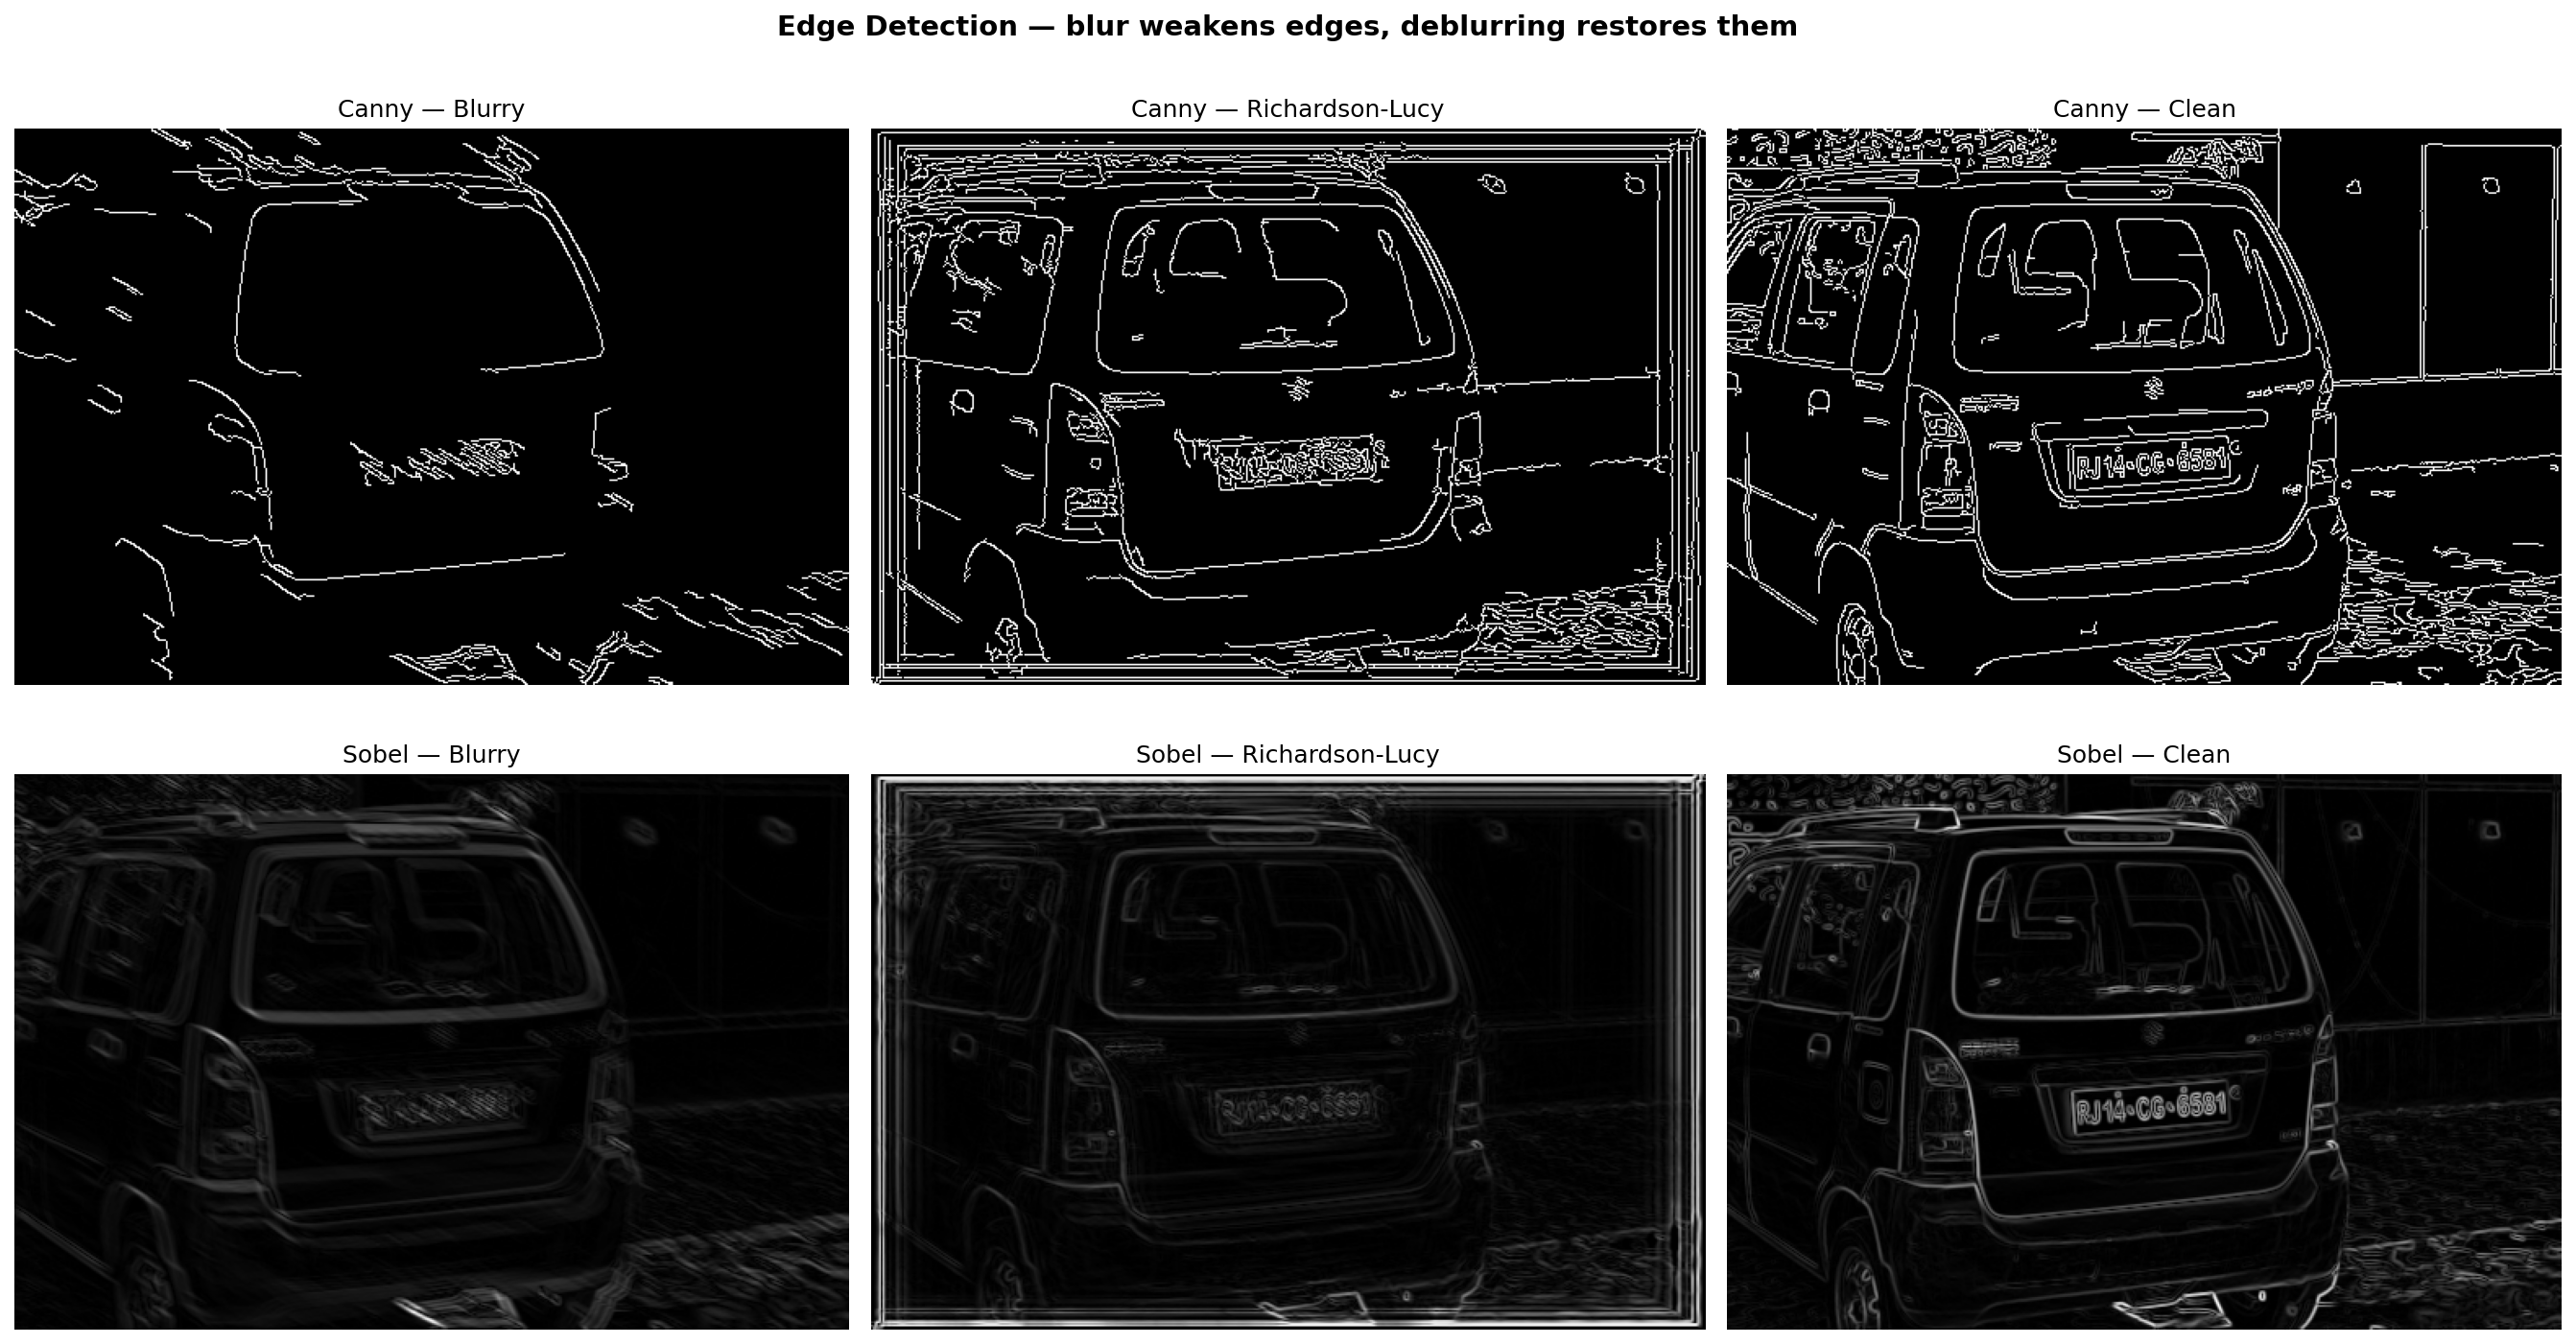
\includegraphics[width=0.55\textwidth,height=0.4\textheight,keepaspectratio]{../outputs/figures/edge_comparison.png}
\caption{\small Canny/Sobel edges: restoration recovers gradient structure, fidelity is lower}
\end{figure}
\end{frame}

% ---- 12: Limitations & Future Work ----
\begin{frame}{Limitations \& Future Work}
\textbf{Gaps we acknowledge:}
\begin{itemize}\setlength{\itemsep}{2pt}
  \item[\textbf{(1)}] \textbf{No OCR evaluation.} PSNR/SSIM $\ne$ plate readability.
  \item[\textbf{(2)}] \textbf{Oracle sweep limited to 1 image.} Full motion-set oracle sweep is next.
  \item[\textbf{(3)}] \textbf{No blur-type classifier.} Single motion PSF applied to all inputs.
  \item[\textbf{(4)}] \textbf{TV ablation not quantified.} Implemented but not A/B-tested.
  \item[\textbf{(5)}] \textbf{No variance reporting.} Means only; no std / CI.
\end{itemize}

\vspace{0.3cm}
\textbf{Natural next steps:}
\begin{itemize}\setlength{\itemsep}{2pt}
  \item Tesseract / EasyOCR CER on blurry vs.\ restored
  \item Multi-scale / adaptive PSF estimation
  \item Real surveillance footage; blur-type classifier upstream
\end{itemize}
\end{frame}

% ---- 13: Thank You ----
\begin{frame}
\begin{center}
\Huge \textbf{Thank You!}

\vspace{1cm}
\large Questions?

\vspace{1cm}
\normalsize
Hamza Ziouine \& Leonce Theureau \\
Group Opus \\[0.2cm]
\small Universit\'e Internationale de Rabat --- April 2026
\end{center}
\end{frame}

\end{document}
